\section{Methodology}

The dataset includes voice measurements from 31 individuals, 23 with
Parkinson's disease, across 195 recordings. The recordings are labeled as 0 for
healthy and 1 for Parkinson's. Features include: absJitter, apq, apq3, apq5,
avFF, dda, dbShimmer, ddp, D2, DFA, HNR, lShimmer, maxFF, minFF, NHR,
percJitter, PPE, ppq, rap, RPDE, spread1, and spread2.

We began with an exploratory analysis and found no missing values, NaNs, or
duplicates. Preprocessing included: renaming columns using \texttt{rename()}
for consistency; removing outliers with \texttt{outliers()} based on the IQR
method \((Q3 - Q1)\), replacing them with the mean per subject to preserve
within-subject consistency; aggregating trials per subject using
\texttt{aggregate()} to compute mean feature values; and applying Min-Max
scaling via \texttt{normalize()}.

For the KNN model, we conducted dimensionality reduction, focusing on
parameters related to fundamental frequency, jitter, and shimmer. The
\texttt{collinearity()} function calculated correlations within each feature
group and identified the least correlated pairs. To retain a feature, we
compared its correlation with all other features. A scoring system assigned
higher scores to features with lower overall correlation. Features with higher
scores were kept, while others were removed.

\begin{figure}[H]
	\centering
	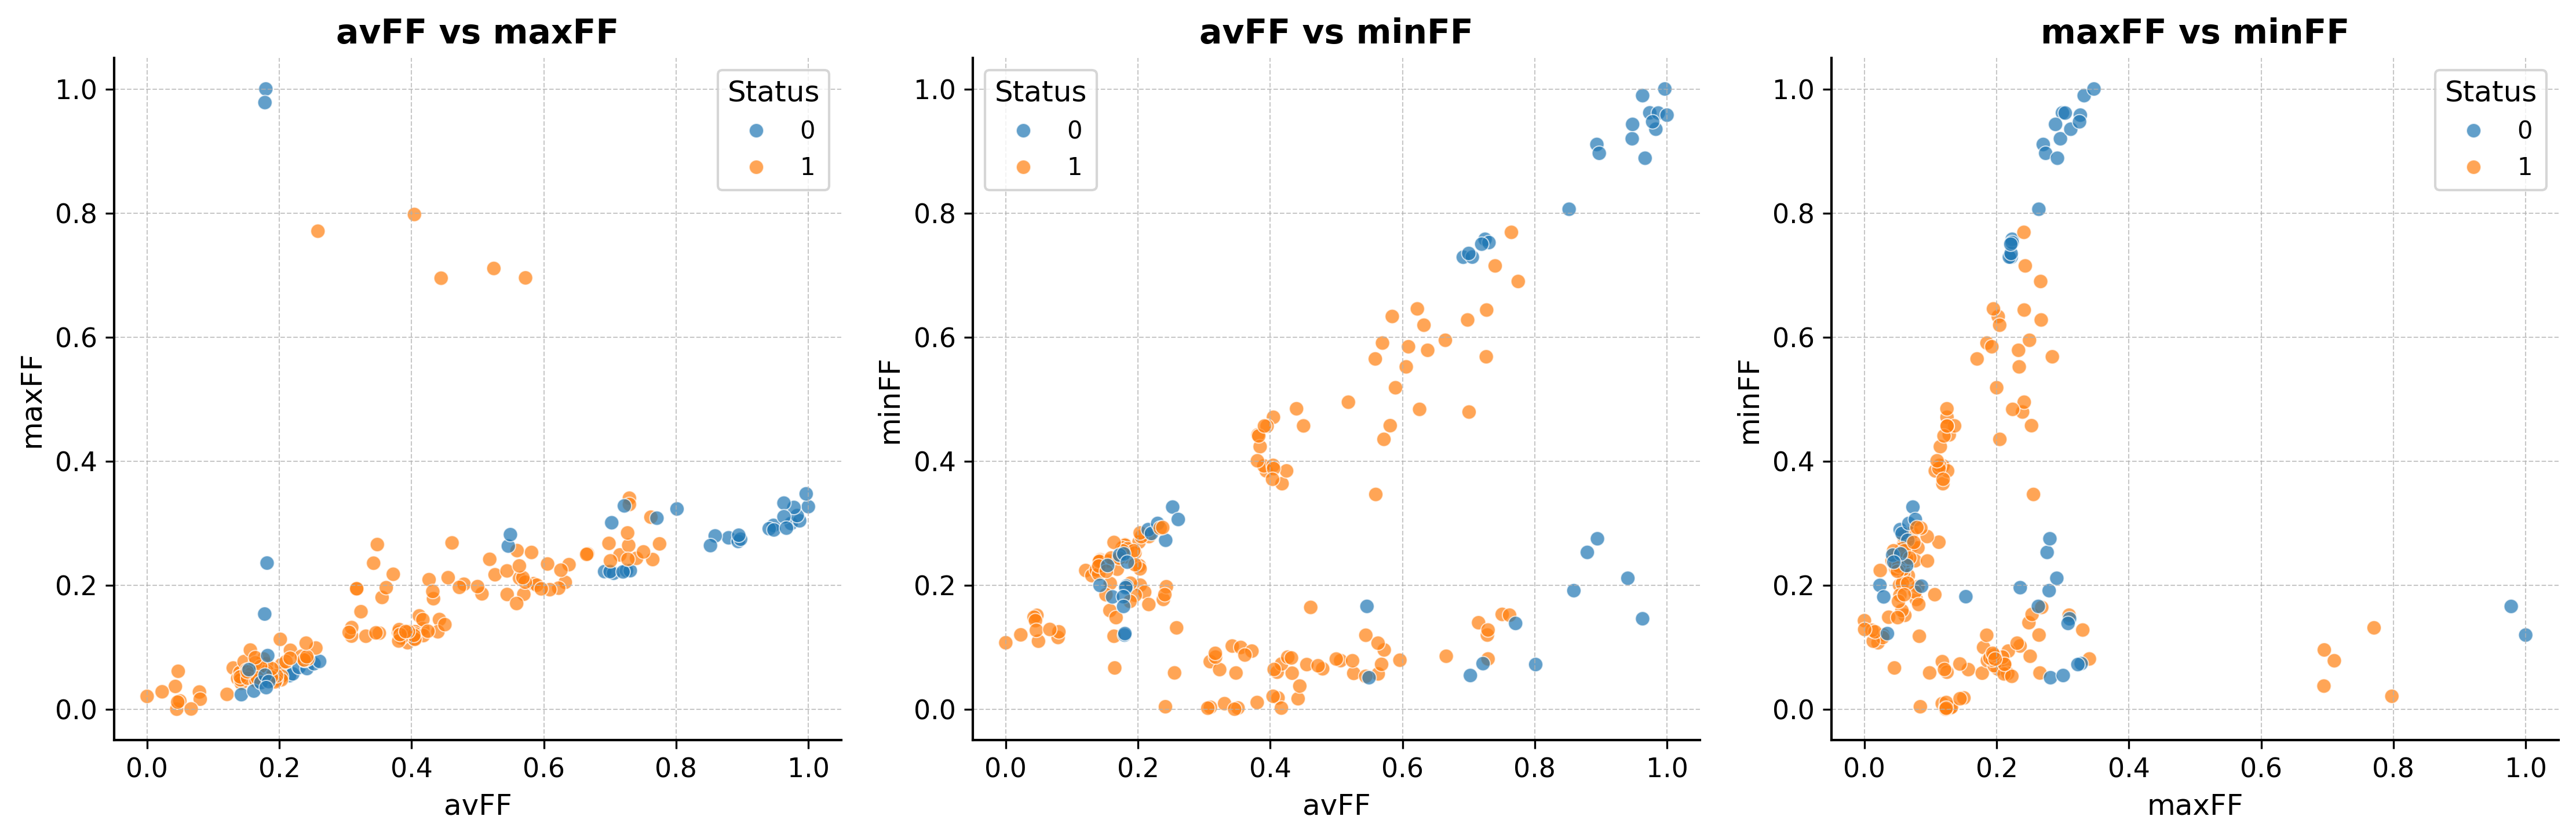
\includegraphics[width=0.99\textwidth,height=6cm]{../images/feature_selection/fundamental_frequency.png}
	\caption{Correlation among fundamental frequency-related parameters.}
	\label{fig:fig2}
\end{figure}

\cref{fig:fig2} shows correlations for fundamental frequency features. As you
can see, since these metrics are relative to the same measure, it makes sense
that they show some sort of correlation between them. The final selected
features to train the model were: absJitter, apq, D2, DFA, HNR, maxFF, NHR,
PPE, RPDE, spread1, spread2.

For validation, the data was split into 70\% training and 30\% testing. To
optimize the hyperparameter \(k\), we selected the value where testing and
training accuracy were similar. The intersection of these points was found
using linear interpolation in the \texttt{best\_k()} function.
